% v1.7 - 2014-11-18
% - bib fixes: now using biber instead of bibtex (thanks felix)
% - compile now with pdflatex -> biber -> pdflatex
% v1.6 - 2013-05-13
% - bibliography headers fixed - thanx lorenz lehmann
% - high quality titlepage - thanx thomas graf
% - removed separation of online and offline references -> style 1.4a
% v1.5 - 2013-01-16

\documentclass[twoside,11pt,titlepage,a4paper,english,bibliography=totocnumbered,listof=numbered]{scrbook}

% Template Style
\include{style}
\addbibresource{main.bib}

% custom hyphenation					% add words to this list to prevent hyphenation
\hyphenation{
ASCII
TCP
}

%make readable references
\usepackage[pdftex,pdfpagelabels=true,hidelinks]{hyperref}
\hypersetup{%
	pdftitle={Indoor Navigation},
	pdfauthor={Lennart, Jan, Eridy, Andreas },
	pdfkeywords={navigation, indoor, indoor navigation, ios, android, nodejs},
	pdfsubject={Indoor Navigation}
}


\begin{document}

%--------------------------------------------------------------
\frontmatter

\begin{titlepage}
	\AddToShipoutPicture*{
		\put(0,0){
			\includegraphics[width=\paperwidth,height=\paperheight,keepaspectratio=false]{images/titlepage.pdf}
		}
	}
	\strut
	\hfill
	\begin{center}
	\vspace{1cm}
		\Huge
		\begin{spacing}{.9}
			\textcolor{DarkRed}{\textbf{Indoor Navigation}}\\
		\end{spacing}
		\vspace{0.8cm}
		\large
		by\\
		\vspace{0.8cm}
		\textbf{Lennart (XXXXXXX)\\ Jan (XXXXXX)\\ Eridy (XXXXXXX)\\ Andreas (XXXXXXX)}\\
		\vspace{2cm}
	 	A project documentation submitted to\\
		\vspace{0.5cm}
		Technische Universität Berlin\\
		School IV - Electrical Engineering and Computer Science\\
		Department of Telecommunication Systems\\
		Service-centric Networking\\
		\vspace{0.5cm}
		Project Documentation\\
		\vspace{2.2cm}
		\today\\
		\vspace{2.0cm}
		\large
		Supervised by:\\
		Sebastian Zickau and Mathias Slawik\\
		\vspace{1cm}
		\end{center}
         		%\includegraphics[scale=1.0]{images/watermark.png}
\end{titlepage}
\thispagestyle{empty}

\cleardoublepage

\newpage

\chapter*{Abstract}
\label{cha:abstract}

Short summary of project outcome.
\thispagestyle{empty}

\tableofcontents{\thispagestyle{empty}}

%--------------------------------------------------------------
\mainmatter

%\part{}						% optional: use parts to structure your thesis
\chapter{Introduction}
\label{cha:introduction}

Motivation:
\begin{itemize}
    \item Write down what the idea behind our project was
    \item Include the use case images and explain them
    \item State constraints and requirements
\end{itemize}

\hline


\begin{center}
    \includegraphics[width=\textwidth]{mensa}\\
    The mensa in Hardenbergstraße at TU Berlin.
\end{center}

\begin{center}
    \includegraphics[width=\textwidth]{use-case-mensa-people}\\
    Yellow person looking for her/his friends in crowded mensa.
\end{center}

\begin{center}
    \includegraphics[width=\textwidth]{use-case-tablet}\\
    Imagined use of our app on mensa tray.
\end{center}

\begin{center}
    \includegraphics[width=\textwidth]{user-story}\\
    Steps on user's way to her/his friends.
\end{center}
\chapter{Related Work}
\label{cha:relatedwork}


We are now going to take a look into what technology is available to accomplish our project goals defined in the previous chapter. First, we are starting with an overview of localization technologies that are in the reach of our project. After that we evaluate which ones are suitable for the circumstances our project is positioned in. And at the end one specific available solution will be examined more deeply in order to determine its possible value for our implementation.


\vspace{0.5cm}

\section{Projects With Same Idea}


\vspace{0.5cm}

\section{Localization Technologies}

\subsection{Estimote Beacons}
Estimote Beacons and Stickers are wireless sensors that can be attached to any location or object, embodying a wireless sensor network. The Beacons consists of a 32-bit ARM Cortex CPUs, equipped with an accelerometer, temperature sensor and a 2.4 Ghz radio. Using Smart Bluetooth 4.0.(Bluetooth low energy), the beacons send out signals with a range of up to 70 meters (Beacons) and 15 meters (Stickers). Though the signals are oftenly distracted under real world conditions, a range of about 40-50 and (Beacons) can be suspected. The battery can as stated by  \cite{developerDocsEstimote} last more than 3 years on default settings on a single CR2477 battery.

Estimote beacons are working with the Apple iBeacon protocol as well as the Eddystone  open beacon format introduced by Google. These protocols working on top of the BLE technology standard are implemented in all smartphones devices enabling them to support new technologys like Apple Watch or Fitness trackers.

Using the Estimote SDK \cite{developerDocsEstimote} mobile applications are enabled to receive and understand BLE Estimote signals in order to calculate the proximity to nearby locations and objects. The beacons specifics provide informations about their type, ownership and approximate locations, temperature or motions.

By the detecting a beacon signal a phone can estimate the distance by measuring the received signal strength \cite{developerDocsEstimote} Since Bluetooth Low Energy does not need any pairing process between sender and receiver, the phone can constantly process new signals. this opens the doors for new technologic opportunities as indoor location/ indoor positioning.

\subsubsection{IBeacon Protocol}
The iBeacon protocol is a Bluetooth low energy communication protocol developed by Apple Inc. in 2013 and was introduced in iOS7 for indoor navigation. The protocol is supported by iOS7 devices as well as Android from version 4.3 up. The signal which is sent by a beacon is called advertisement. 

These advertisements provides a so called iBeacon identifier, that is is 20 bytes long and divided into three sections:

\begin{itemize}
\item UUID (16 bytes)
\item major number (2 bytes)
\item minor number (2 bytes)
\end{itemize}


These values provided by the advertisement can be modified according to own wishes.
The hierarchical configuration of these values provides identifying informations about the beacon. While the UUID can be destinguished to a corporation, major and minor values can be used to distinguish between regions and sub-regions of a corporation.

\subsubsection{Region Monitoring}
Region monitoring triggers actions on the device on entering or exiting a beacon defined regions range. This works in depending the devices capabilities while an app is in foreground background or suspended. An app is limited to 20 regions being monitored. However by using a single UUID in multiple locations, a device can monitor many physical locations simultaneously \cite{appleIBeacon}.

\subsubsection{Ranging}
Ranging however triggeres actions on the devise based on the proximity to a beacon.
The iBeacon protocol applies filters to the accuracy of a advertisement of one beacon. The filterestimation regarding the proximity to a beacon is indicated using one of four proximity states.

\begin{itemize}
\item Immediate \\
The Immediate proximity state represents a high level of confidence, that the device is physically very close to the beacon. This is in example holding the Smartphone directly on to of a beacon.
	
\item Near \\
The Near proximity state indicates a proximity of round about 1-3 meters, if there are no obstructions between the device and the beacon which might cause distractions of the beacon.

\item Far \\
The Far proximity state indicates a detected beacon without much confidence in the accuracy that is to low to determine wether it is Near or Immediate. The Far proximity state relies on the accuracy property to determine the potential proximity to the beacon.


\item Unknown\\
The Unknown proximity state indicates a state where beacons are can not be determined. This my happen if the ranging has just begun or that the accuracy level is insufficient for measurements to determine a state that is either Far, Near or Immediate.
\end{itemize}

\subsubsection{Estimote Beacon Drawbacks}
For the implementation of Estimote Indoor Navigation for the project we decided to use Monitoring on the devices in order to detect the beacons, specifiyng a certain region. However, the devices still take at least about 30 seconds to recognize the fact that a beacon is out of range. This is a  built-in and non adjustable delay in order to prevent "false" exit events.\cite{developerDocsEstimote} This is a major drawback regarding a use-case of the project, that a user might pass multiple beacons of a location and constantly update new locations without the need to stop at each beacon.

This is solved by in additional applied ranging of all beacons that are monitored in order to process the "nearest" beacon as a users location. The devices report then the beacons in an order that is best guess of their proximity regarding issues of signal attenuation. This order however may still not be correct.\cite{appleIBeacon}

\subsubsection{Apple Core Location Framework}
As firstly presented on WWDC2015 \cite{wwdc15}  Apple presented new functionalities to the already existing Core Location Framework which is the major Framework on iOS devices for location service \cite{CLlocation}. This Framework takes the user in charge of wether the app can use locations services on the device or not.

The Core Location Framework uses Cellular data to provide an aproximity in which area in a city a user is. Additionally it uses GPS based on Satellite signals to improve the position of the user as well as sorounding Wi-Fi signals.

As soon as the user enters an indoor venue, the iOS system turns down GPS and Cellular sensors and enlightens Motion and Wi-Fi sensors. 
These sensors are used in combination with the remaining GPS signals, comming through the windows to locate the user indoors. The Motion sensor hereby gives information to the system that a person is moving and how fast the user is moving, while wi-fi signals are feeded to the CLLocation Framework to calculate the exact position.

Apple also added the altitude and floor attributes to the CLLocation Framework in order to provide the user with the correct floor attributes \cite{CLlocation}.

For the Project the new CLLocation Framework was used to show the users Positon in the Mensa. After the first indoor tests in the mensa revealed precise positioning of a user indoors. However the Framework also revealed large susceptibility in areas where the wi-fi signal was apparently weak. i.e. in the upper left corner of the Mensa which is surrounded by walls that are affecting the router wifi signals.

The Frameworks started in an early beta when this project started and is constantly improved. To enable the full abilities of CLLocation Framework indoors, the venue needs to be registered and enabled by apple, using Maps Connect program \cite{mapsConnect} in order to unlock CLLocation Frameworks full potential.

\vspace{0.5cm}

\section{Evaluation of Available Technologies}


\vspace{0.5cm}

\section{CISCO MSE API Wrapper Tests}

In order to determine whether the CISCO MSE API wrapper provided by tubIT would be sufficient for the project's requirements we were asked to perform tests on it. Especially it was asked for details on how the API worked where, so what values could be retrieved via the API wrapper in which locations on campus and how precise the values would turn out to be.

Concerning use cases our project was focused on the mensa and the library, therefore we initially planned to be conducting tests in only these two locations. As the provided wrapper around the CISCO MSE API we had access to delivered back one short, simple XML line we decided to invest some time into developing a small tool which routinely queried the API for it's current status and saved the result into an easily readable JSON file for later investigation. The source code of the developed tool you can find in appendix \ref{appendix:cisco-mse-api-test}.

\begin{center}
    \includegraphics[width=\textwidth]{cisco-mse-api-response}\\
    What the CISCO MSE API wrapper response looks like.
\end{center}

It was planned to be conducting the tests on one day in the mensa and on another day in the library. On the first day we started around noon and ran the test tool on one of our notebooks connected to university WiFi, \enquote{eduroam}. We started in the south-western corner near the windows, walked towards the south-eastern corner, went to the stairs in the northern part and upstairs and again at the window front to the south-western corner on the first floor. As it turned out, the results we got back were definitely not what we had hoped for, most importantly because longitude and latitude of the requesting user were missing completely. The following listing shows the first ten results logged in two second periods from the API wrapper:

\begin{lstlisting}
{
    "signal": [
        {"timestamp": 1445344391, "latitude": "0.000000000000000", "longitude": "0.000000000000000", "building": "Mensa", "floor": "Mensa 1. OG"},
        {"timestamp": 1445344393, "latitude": "0.000000000000000", "longitude": "0.000000000000000", "building": "Mensa", "floor": "Mensa 1. OG"},
        {"timestamp": 1445344395, "latitude": "0.000000000000000", "longitude": "0.000000000000000", "building": "Mensa", "floor": "Mensa 1. OG"},
        {"timestamp": 1445344397, "latitude": "0.000000000000000", "longitude": "0.000000000000000", "building": "Mensa", "floor": "Mensa 1. OG"},
        {"timestamp": 1445344399, "latitude": "0.000000000000000", "longitude": "0.000000000000000", "building": "Mensa", "floor": "Mensa 1. OG"},
        {"timestamp": 1445344401, "latitude": "0.000000000000000", "longitude": "0.000000000000000", "building": "Mensa", "floor": "Mensa 1. OG"},
        {"timestamp": 1445344404, "latitude": "0.000000000000000", "longitude": "0.000000000000000", "building": "Mensa", "floor": "Mensa 1. OG"},
        {"timestamp": 1445344406, "latitude": "0.000000000000000", "longitude": "0.000000000000000", "building": "Mensa", "floor": "Mensa 1. OG"},
        {"timestamp": 1445344408, "latitude": "0.000000000000000", "longitude": "0.000000000000000", "building": "Mensa", "floor": "Mensa 1. OG"},
        {"timestamp": 1445344410, "latitude": "0.000000000000000", "longitude": "0.000000000000000", "building": "Mensa", "floor": "Mensa 1. OG"},
        ...
    ]
}
\end{lstlisting}

Clearly it can be observed that the longitude and latitude values are unusable. Another take away was that the floor change during our test did not reflect into our captured results. Therefore we decided to directly test the library for comparable results. Inside the library, we started on ground floor and went upstairs in \enquote{circles} through the different levels. From the fourth floor we went back down straight forward. During that second test ten of the first fifteen responses from the API looked like:

\begin{lstlisting}
{
    "signal": [
        {"timestamp": 1445345843, "latitude": "0.000000000000000", "longitude": "0.000000000000000", "building": "BIB", "floor": "Erdgeschoss"},
        {"timestamp": 1445345845, "latitude": "0.000000000000000", "longitude": "0.000000000000000", "building": "BIB", "floor": "Erdgeschoss"},
        {"timestamp": 1445345848, "latitude": "0.000000000000000", "longitude": "0.000000000000000", "building": "BIB", "floor": "Erdgeschoss"},
        {"timestamp": 1445345850, "latitude": "0.000000000000000", "longitude": "0.000000000000000", "building": "BIB", "floor": "Erdgeschoss"},
        {"timestamp": 1445345852, "latitude": "0.000000000000000", "longitude": "0.000000000000000", "building": "BIB", "floor": "Erdgeschoss"},
        {"timestamp": 1445345854, "latitude": "0.000000000000000", "longitude": "0.000000000000000", "building": "BIB", "floor": "Erdgeschoss"},
        ...
        {"timestamp": 1445345870, "latitude": "0.000000000000000", "longitude": "0.000000000000000", "building": "BIB", "floor": "1. Obergeschoss"},
        {"timestamp": 1445345872, "latitude": "0.000000000000000", "longitude": "0.000000000000000", "building": "BIB", "floor": "1. Obergeschoss"},
        {"timestamp": 1445345874, "latitude": "0.000000000000000", "longitude": "0.000000000000000", "building": "BIB", "floor": "1. Obergeschoss"},
        {"timestamp": 1445345876, "latitude": "0.000000000000000", "longitude": "0.000000000000000", "building": "BIB", "floor": "1. Obergeschoss"},
        ...
    ]
}
\end{lstlisting}

First, longitude and latitude were again unusable. This time though the floor information worked quite reliably and indicated very fast on which floor we currently measured. After that we were wondering whether eventually we would get back longitude and latitude values anywhere on campus and decided to give it one last try by taking one more measurement in the MAR building (Marchstraße).

One more measurement turned into three as during the first two attempts we got sudden disconnects and therefore unusable results. We walked the whole foyer from north to south side and somewhere near the entrance we suspect the wireless signal got bad and our notebook conducting the tests disconnected. In the third try though we finally were able to get back usable results, in which chosen ten results logged looked like this:

\begin{lstlisting}
{
    "signal": [
        {"timestamp": 1445350550, "latitude": "52.516903688639005", "longitude": "13.323958376544699", "building": "MAR", "floor": "Erdgeschoss"},
        {"timestamp": 1445350552, "latitude": "52.516903688639005", "longitude": "13.323958376544699", "building": "MAR", "floor": "Erdgeschoss"},
        {"timestamp": 1445350554, "latitude": "52.516903688639005", "longitude": "13.323958376544699", "building": "MAR", "floor": "Erdgeschoss"},
        {"timestamp": 1445350557, "latitude": "52.516903688639005", "longitude": "13.323958376544699", "building": "MAR", "floor": "Erdgeschoss"},
        ...
        {"timestamp": 1445350686, "latitude": "52.516864921942748", "longitude": "13.323953890659670", "building": "MAR", "floor": "Erdgeschoss"},
        {"timestamp": 1445350688, "latitude": "52.516864921942748", "longitude": "13.323953890659670", "building": "MAR", "floor": "Erdgeschoss"},
        {"timestamp": 1445350690, "latitude": "52.516864921942748", "longitude": "13.323953890659670", "building": "MAR", "floor": "Erdgeschoss"},
        ...
        {"timestamp": 1445350845, "latitude": "52.516402095317481", "longitude": "13.323531401046099", "building": "MAR", "floor": "Erdgeschoss"},
        {"timestamp": 1445350847, "latitude": "52.516402095317481", "longitude": "13.323531401046099", "building": "MAR", "floor": "Erdgeschoss"},
        {"timestamp": 1445350849, "latitude": "52.516402095317481", "longitude": "13.323531401046099", "building": "MAR", "floor": "Erdgeschoss"},
        ...
    ]
}
\end{lstlisting}

Finally we received some longitude and latitude values. Unfortunately the three different pairs of longitude and latitude above were the only ones we could observe during the whole walk from north end to south end of the foyer, thus still rather unusable values.

In the end, our conclusion at that point in the project progress was to use the CISCO MSE API wrapper provided by the tubIT in order to retrieve the rough position of a user. This means the building and floor the request originated from. We recommended back to our supervisors not to use this API for receiving longitude and latitude as these values were either quite imprecise or not available at all. The full result files of all our three measurements can be found at \cite{ioslINavGitHub}.
\chapter{Concept and Design}
\label{cha:conceptanddesign}

Explain what defines our concept (setup):
\begin{itemize}
    \item Big picture setup explanation
    \item API format (RESTful JSON API)
    \item Client side vs. server side
    \item Authentication idea
    \item Database design
    \item etc...
\end{itemize}


\vspace{0.5cm}

\section{Big Picture}

As already mentioned our system will consist of two parts, the mobile clients side and the backend side which interconnectedly exchange data. The backend part itself is split up again in three parts of which one is an \enquote{external} (means: SNET) resource, the CYCLONE Federation Provider. This entity provides us with user management and session handling functionalities so that we are able to out source these tedious and error-prone tasks to them. On the other side CYCLONE profits from our experiences with its rather young service. Concerning our part of the backend side, the task was to serve two machines independently, the API server and the database server. This was expected to be achieved with Docker.

To gain an understanding of what system we were trying to build, the following image should be at help:

\begin{center}
    \includegraphics[width=\textwidth]{system-overview}\\
    All components of our envisioned system working together.
\end{center}

To sum it up, the idea is to gather position information aligned to the user's preferences locally on the smartphone, preform some processing steps on it, contact our backend for which authentication via the CYCLONE Federation Provider is needed and after that create, read, update or delete information (CRUD principle) in the backend and therefore in the database.


\vspace{0.5cm}

\section{API Considerations}

We had to decide on which paradigm our API should be based on. The client-server and stateless nature in combination with the just mentioned approach of relying on HTTP verbs such as POST, GET, PUT and DELETE for the CRUD operations, the decision to go for a RESTful API was quite clear (see chapter five \cite{fielding2000architectural}).


\vspace{0.5cm}

\section{Workload Split Between Clients and Server}


\vspace{0.5cm}

\section{Authentication and Session Management}


\vspace{0.5cm}

\section{Database Design}
\chapter{Implementation}
\label{cha:implementation}

Implementation:
\begin{itemize}
    \item Backend architecture
    \item Android
    \item iOS
\end{itemize}


\vspace{0.5cm}

\section{Backend}

\subsection{Architecture}

In this section we will focus on the architecture and our decision for the backend and its communication.
We build a RESTful API which allows the clients to communicate with the backend in a JSON\footnote{\url{http://json.org/index.html}} format. 

\begin{center}
    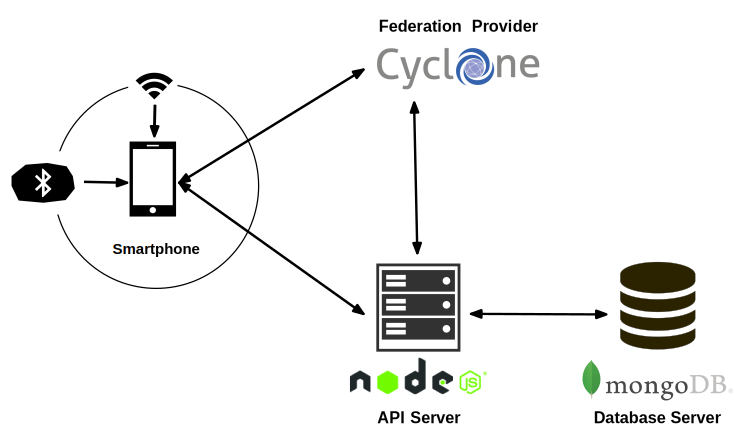
\includegraphics[width=\textwidth]{architecture_v02}\\
\end{center}

\subsection{CYCLONE Federation Provider}

\begin{center}
    \includegraphics[width=\textwidth]{cyclone-federation-provider-login}\\
    Login screen to CYCLONE Federation Provider.
\end{center}


\vspace{0.5cm}

\section{Android}


\vspace{0.5cm}

\section{iOS}

\chapter{Evaluation}
\label{cha:evaluation}

Indoor navigation is a very interesting topic and get more important in context of mobile applications. We researched diffrent technologies for indoor navigation and implemented those in an Android and iOS application. Both devices can locate a user via manual pin pointing on a map,CISCO MSE API and Estimote beacons. First we had really create expectations to the CISCO MSE API but the didn't offer us the longitude and latitude for each building only for some sporadic buildings. So we only could use it for a rough localication of a user. The Estimote beacons give us quite nice expectations on the range from the datasheet but we didn't get the specified range and after sometime the get really bad until the stopped working. We found out that the battery was empty. So we changed it and the worked again but according to the datasheet the beacons should work near to three years without changing the battery.

We had some struggle at the beginning what is possible on the devices and what can we really implement on iOS and Android. We had some specific implementations on both devices like the Apple CLLocation Framework or how we can execute threads in background. The communication between the mobile application is completely in JSON to a RESTful backend in the web. This was very good and useful because we dont had to implement specifics for the devices at the backend.

At the backend we tried to implement some geo-fencing possibilities because the mongoDB should offer us some of these functionalities but the mongoose framework was not implementing it right and we discovered some bugs that hindered us to implement it. The backend technology of nodejs was quite interesting because we had no expirence with an asynchrone programming language but our learning curve was high and it would have been possible that we implement functionalities which are now future work. The CYCLONE Federation Provider was a nice project to include in our work but sometimes we had some struggles with them but mostly to get specific information from the tubIT which we didn't get until now.

In total we dont get everything implemented what we thought we could do at the beginning but we get the main functionalities of sharing a position manuel and automaticaly working on two diffrent devices including the communication to the backend.

%TODO remove itemes below
%Evaluate:
%\begin{itemize}
%    \item What does work so far? What does not?
%    \item What were the observed issues (see final presentation)?
%    \item $\rightarrow$ MSE API, beacons, interplay server with clients, Node.JS, Mongoose (MongoDB), etc.
%\end{itemize}

\chapter{Conclusion}
\label{cha:conclusion}

We did backend, ios, android, docker, nodejs and some other random stuff and now it works


%--------------------------------------------------------------
\backmatter

%\listoftables
\listoffigures

\setwidesite{}						% Set page to be wider for bibliography

\label{cha:bibliography}
\markboth{Bibliography}{Bibliography}
\addcontentsline{toc}{chapter}{Bibliography}
\printbibliography
%\printbibliography[heading=offline,filter=offline]
%\printbibliography[heading=online,filter=online]

\begin{appendices}

\section{PDF Floor plans Mensa}

\begin{figure}[!htb]
\centering
  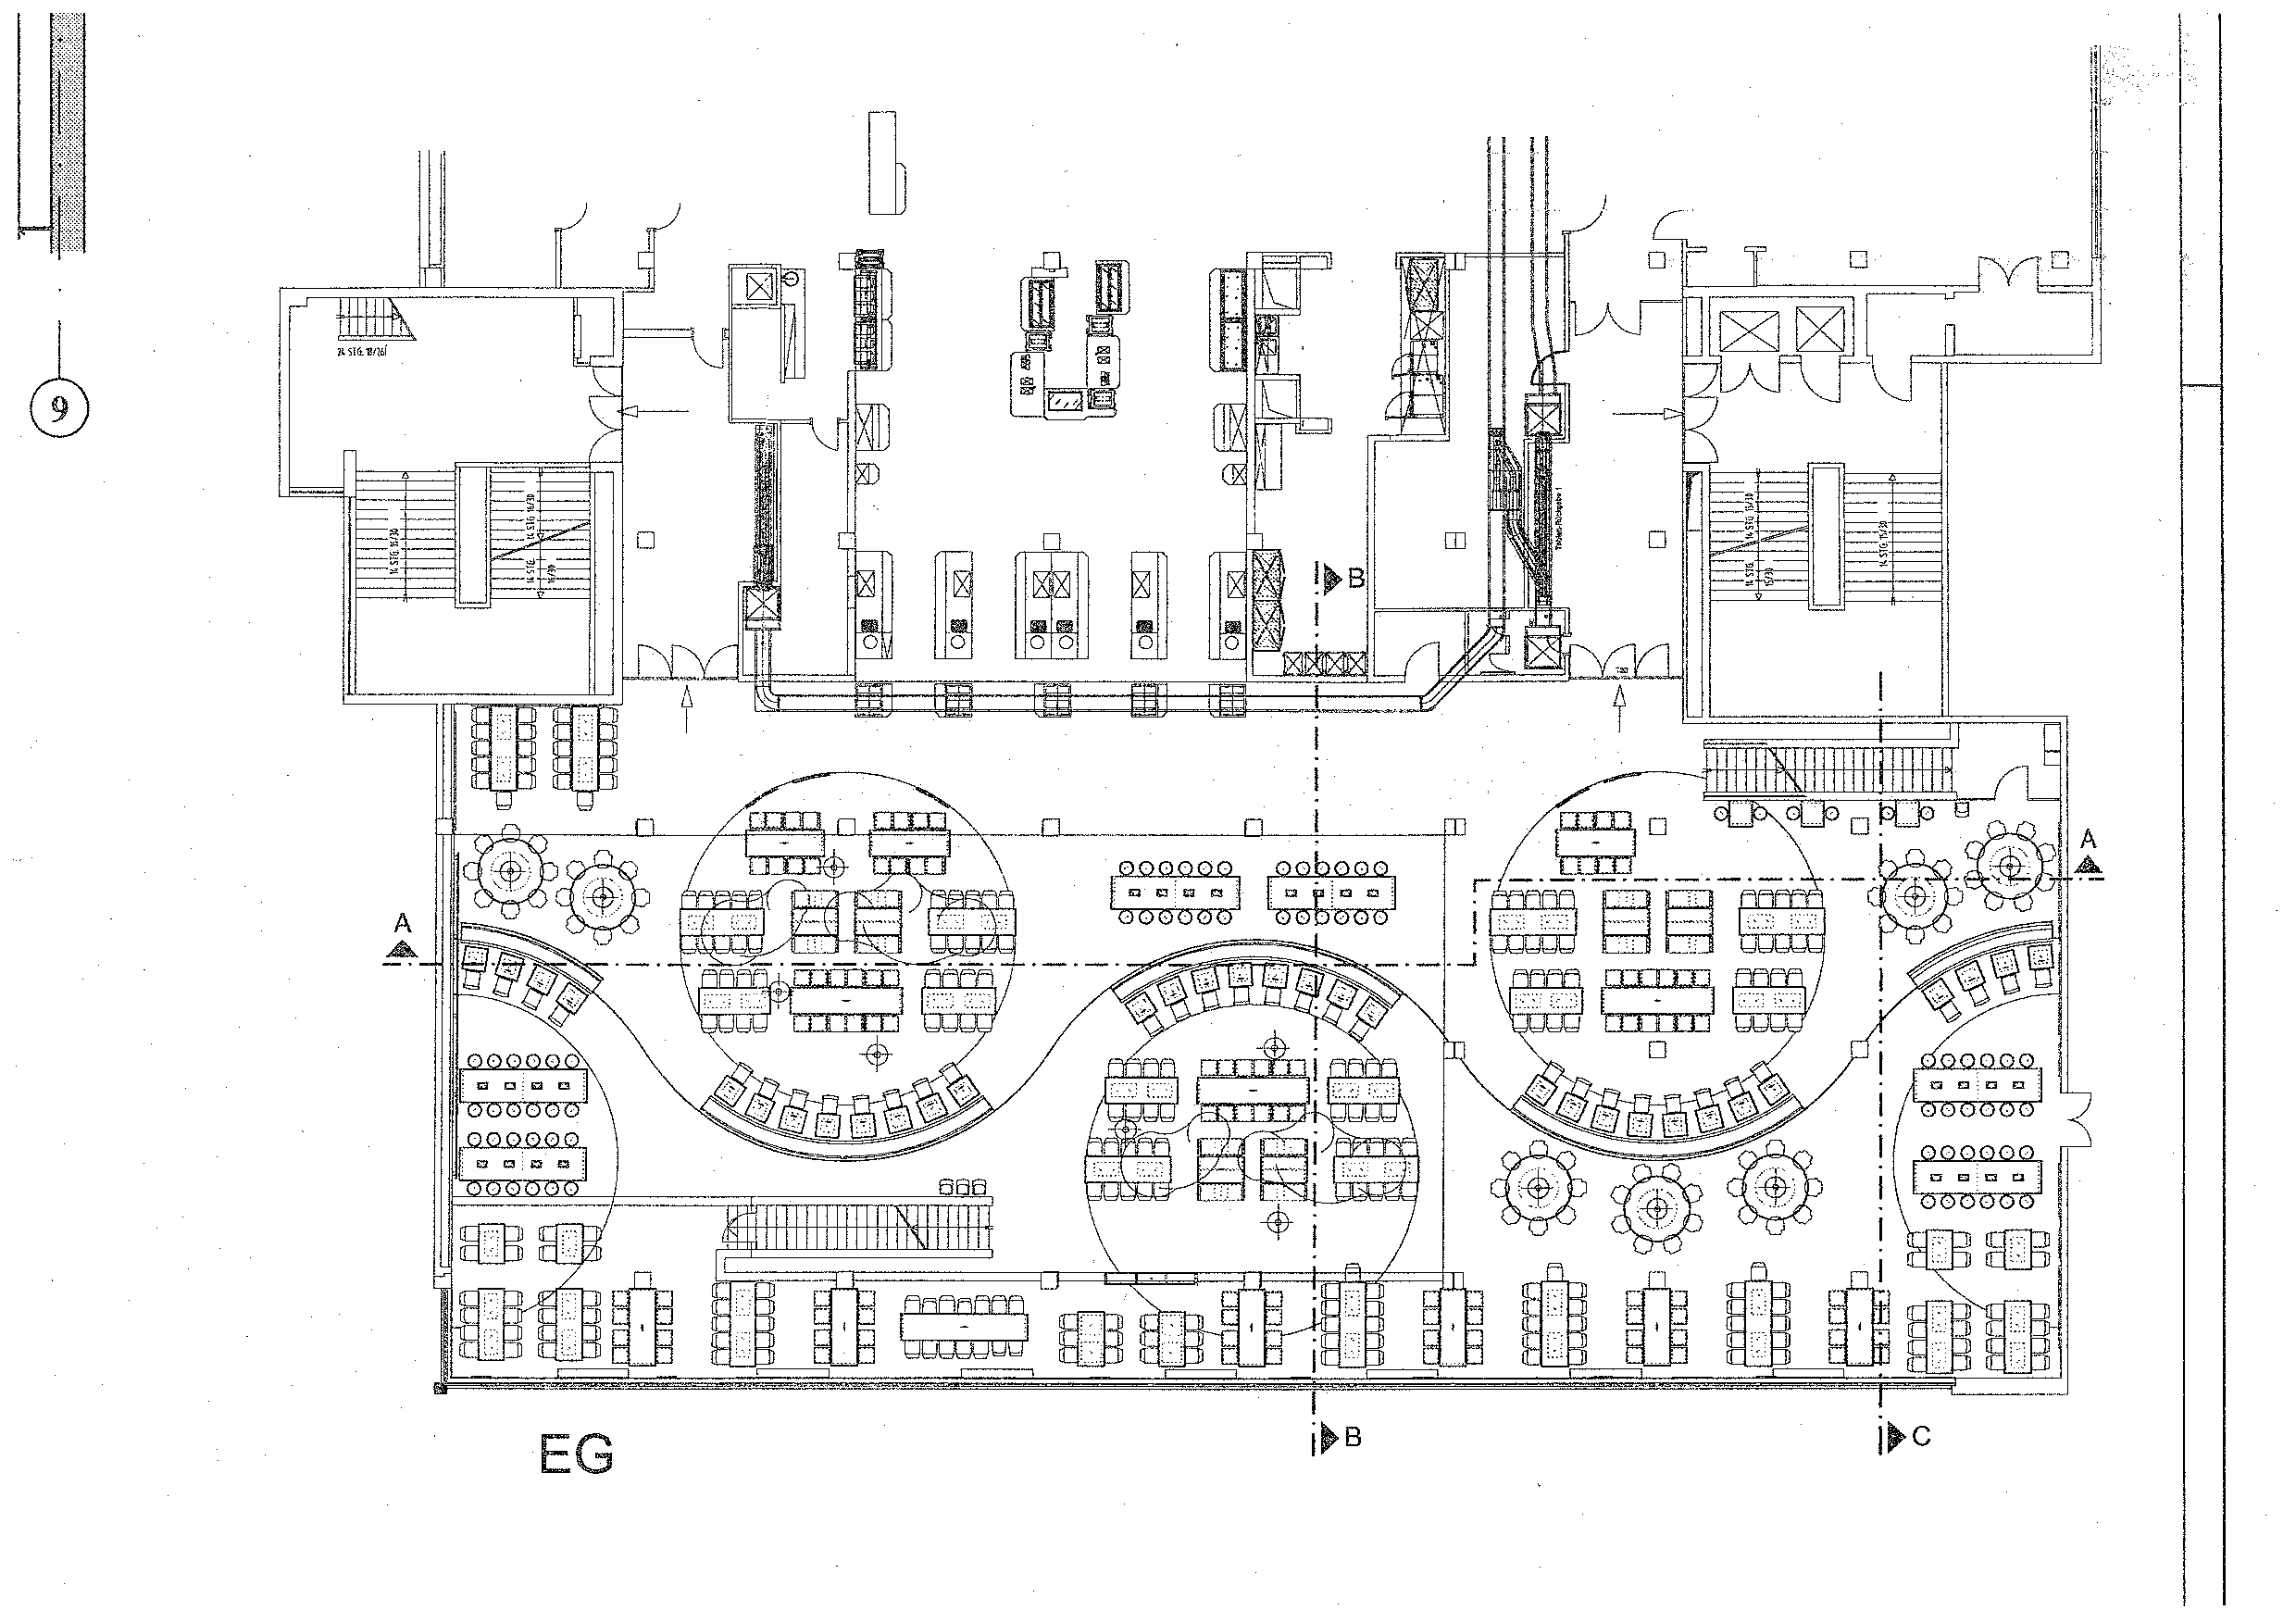
\includegraphics[width=0.75\textwidth]{01_Bestuhlungsplan}
  \captionof{figure}{Floor plan Mensa EG}
\end{figure}

\begin{figure}[!htb]
\centering
  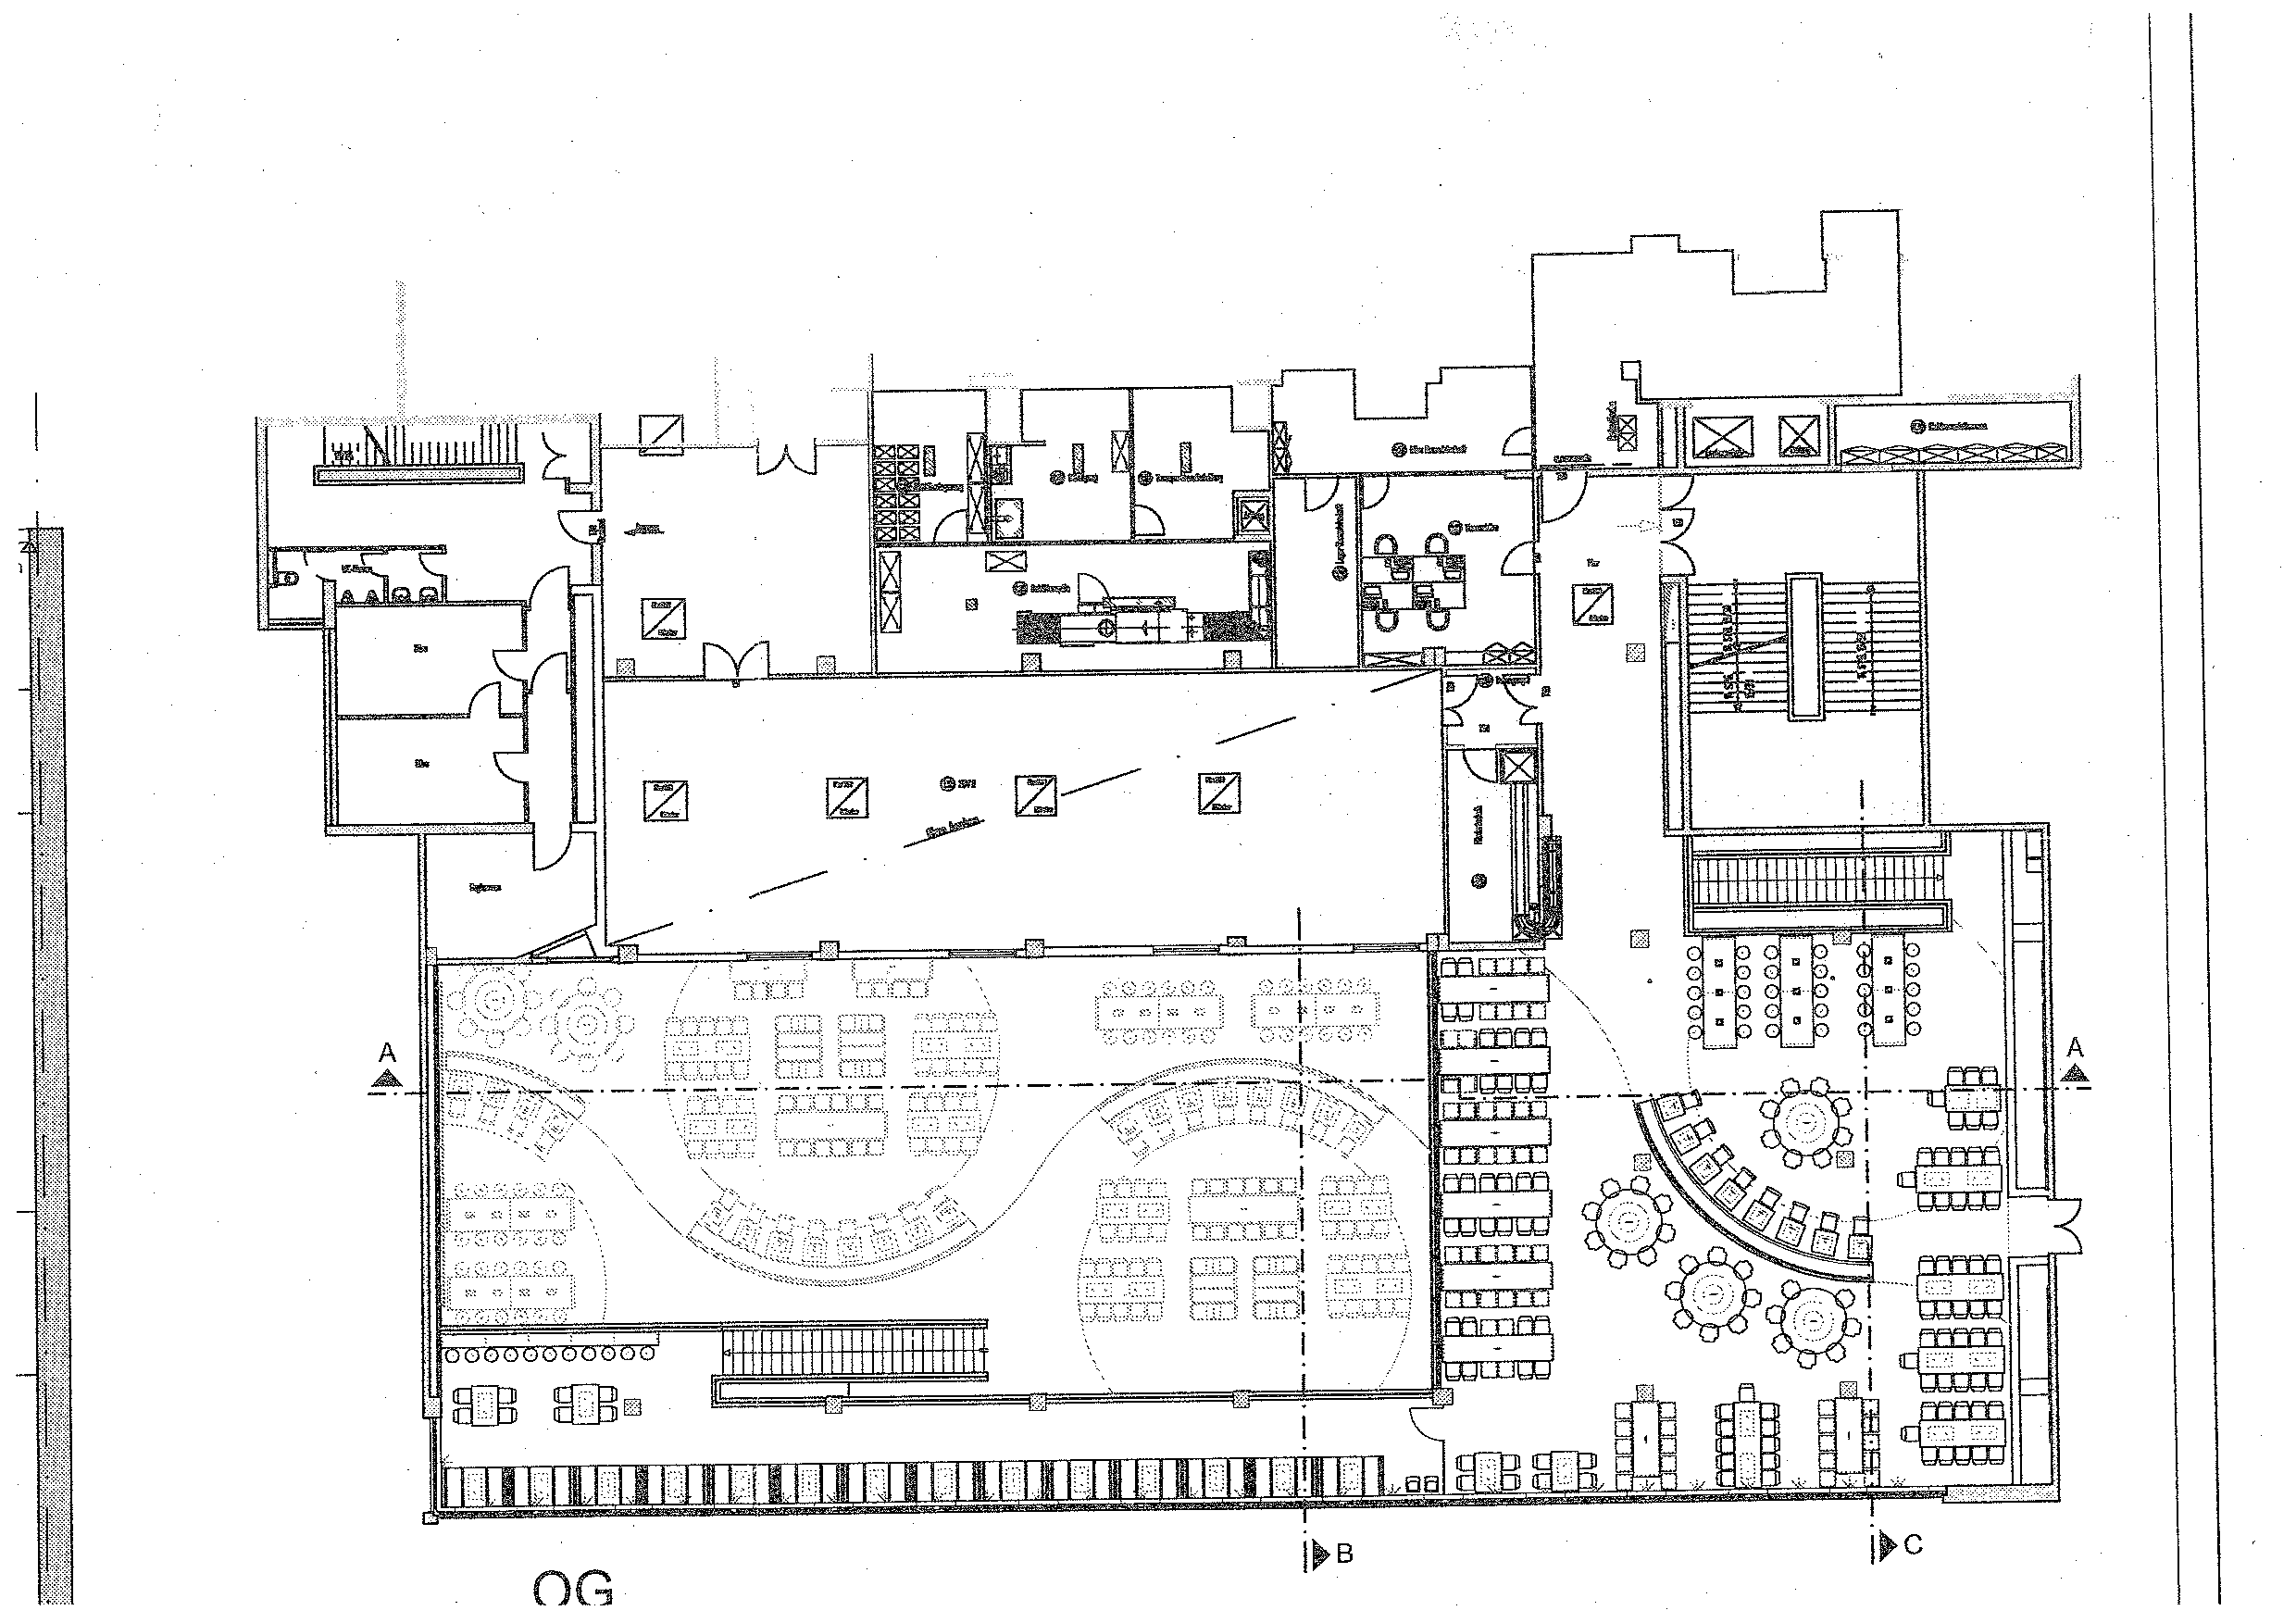
\includegraphics[width=0.75\textwidth]{02_Bestuhlungsplan}
  \captionof{figure}{Floor plan Mensa OG}
\end{figure}

\section{Tool for performing tests on the CISCO MSE API wrapper}
\label{appendix:cisco-mse-api-test}

\begin{lstlisting}[language=go]
package main

import (
    "fmt"
    "log"
    "os"
    "syscall"
    "time"

    "encoding/xml"
    "io/ioutil"
    "net/http"
    "os/signal"
)

type WiFiInfo struct {
    XMLName          xml.Name `xml:"Info"`
    ChangedOn        string   `xml:"changedOn,attr"`
    ConfidenceFactor float32  `xml:"confidenceFactor,attr"`
    Building         string   `xml:"building,attr"`
    Floor            string   `xml:"floor,attr"`
    Network          string   `xml:"WLAN-Status,attr"`
    UserName         string   `xml:"username,atrr"`
    Longitude        float64  `xml:"lon,attr"`
    Latitude         float64  `xml:"lat,attr"`
}

type LogWiFiStruct struct {
    Timestamp int     `json:"timestamp"`
    Latitude  float64 `json:"latitude"`
    Longitude float64 `json:"longitude"`
    Building  string  `json:"building"`
    Floor     string  `json:"floor"`
}

func handleUserExit(signalChannel chan os.Signal) {

    for _ = range signalChannel {

        // Define a useful result file name (format: "wifi-measurement-year-month-day-hour-minute-seconds.json")
        fileName := fmt.Sprintf("wifi-measurement-%s.json", fileNameTime)

        // Open measurement result file
        fileResult, fileError := os.OpenFile(fileName, os.O_CREATE|os.O_RDWR|os.O_APPEND, 0666)

        if fileError != nil {
            log.Fatal(fileError)
        }

        // Close open logging file
        defer fileResult.Close()

        log.Printf("\nWritten measurement values to file %s. Good bye.\n", fileName)

        os.Exit(0)
    }
}

func main() {

    // Put in here the API endpoint to the wifi location service.
    const apiURL = "PUT THE API ENDPOINT IN HERE"

    // Get time data
    startTime := time.Now()
    fileNameTime := startTime.Format("2006-1-2-3-4-5")

    // Define a clean up channel
    signalChannel := make(chan os.Signal)
    signal.Notify(signalChannel, os.Interrupt, syscall.SIGTERM)
    go handleUserExit(signalChannel)

    log.Printf("Starting to measure WiFi API.\n")

    for {

        // Make a GET call on that URL
        apiResp, apiError := http.Get(apiURL)

        if apiError != nil {
            log.Fatal(apiError)
        }

        // Read in all body content we got and close connection
        xmlData, ioError := ioutil.ReadAll(apiResp.Body)
        apiResp.Body.Close()

        if ioError != nil {
            log.Fatal(ioError)
        }

        // Our go struct representation of the tubIT XML
        wInfo := WiFiInfo{}

        // Parse received XML into struct
        xmlError := xml.Unmarshal([]byte(xmlData), &wInfo)

        if xmlError != nil {
            log.Fatal("XML parsing error: %v.\n", xmlError)
        }

        // Get the current UNIX epoch timestamp for logging
        timeResult := time.Now().Unix()

        // Build up the log string
        logResult := fmt.Sprintf("\t\t{\"timestamp\": %d, \"latitude\": \"%.15f\", \"longitude\": \"%.15f\", \"building\": \"%s\", \"floor\": \"%s\"},\n", timeResult, wInfo.Latitude, wInfo.Longitude, wInfo.Building, wInfo.Floor)

        // Write log string to opened file
        fileResult.WriteString(logResult)

        log.Printf("Received: \"long\": %v, \"lat\": %v.\n", wInfo.Longitude, wInfo.Latitude)

        // Let the execution wait for 2 seconds
        time.Sleep(2 * time.Second)
    }
}
\end{lstlisting}

\end{appendices}

\end{document}